\documentclass[tikz,border=8pt]{standalone}
\usepackage{ctex}
\usepackage{amsmath,amssymb,bm}
\usetikzlibrary{arrows.meta,calc,angles,quotes,patterns,positioning,decorations.pathmorphing}
\definecolor{ink}{RGB}{30,43,58}
\definecolor{blue}{RGB}{37,91,166}
\definecolor{orange}{RGB}{219,113,25}
\definecolor{green}{RGB}{39,139,94}
\definecolor{red}{RGB}{192,52,52}
\tikzset{line cap=round,line join=round,body/.style={draw=ink,very thick},
axis/.style={-{Latex[length=2.5mm]},draw=ink,very thick},
vec/.style={-{Latex[length=2.5mm]},draw=blue,very thick},
force/.style={-{Latex[length=2.5mm]},draw=red,very thick},
guide/.style={draw=ink!45,dashed},dim/.style={{Latex[length=2mm]}-{Latex[length=2mm]},draw=ink!75}}

\usetikzlibrary{decorations.pathmorphing}
\tikzset{mass/.style={circle,draw,fill=white,minimum size=7mm},curve/.style={very thick,blue},rope/.style={very thick,blue},ray/.style={very thick,blue,-{Latex}},impulse/.style={very thick,orange,-{Latex}},resistor/.style={thick,decorate,decoration={zigzag,segment length=3mm,amplitude=1mm}}}
\begin{document}
% 1 question-01
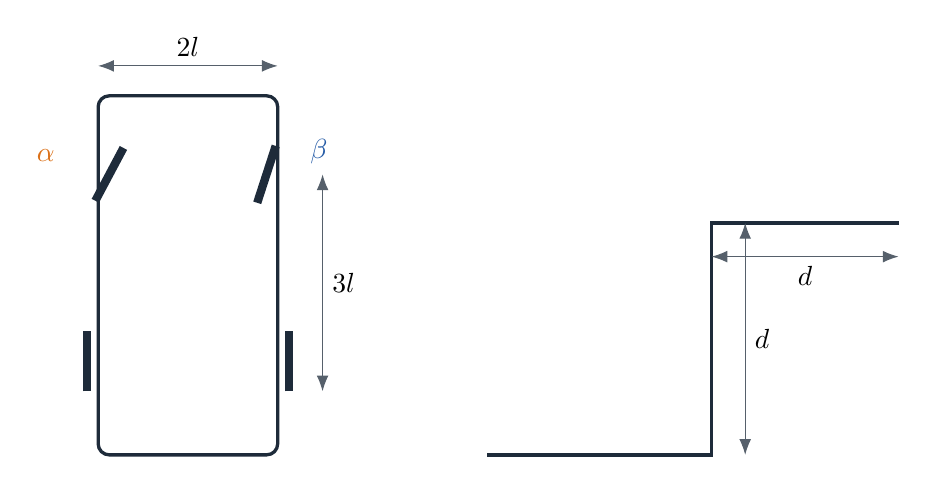
\begin{tikzpicture}[scale=.95]
  \draw[body,rounded corners=4pt] (-1.2,-2.4) rectangle (1.2,2.4);
  \foreach \x in {-1.35,1.35}{\draw[body,line width=3pt] (\x,-1.55)--(\x,-.75);}
  \draw[body,line width=3pt,rotate around={-28:(-1.05,1.35)}] (-1.05,.95)--(-1.05,1.75);
  \draw[body,line width=3pt,rotate around={-18:(1.05,1.35)}] (1.05,.95)--(1.05,1.75);
  \draw[dim] (-1.2,2.8)--(1.2,2.8) node[midway,above] {$2l$};
  \draw[dim] (1.8,-1.55)--(1.8,1.35) node[midway,right] {$3l$};
  \node[orange] at (-1.9,1.6) {$\alpha$}; \node[blue] at (1.75,1.65) {$\beta$};
  \draw[body] (4,-2.4)--(7,-2.4)--(7,.7)--(9.5,.7);
  \draw[dim] (7.45,-2.4)--(7.45,.7) node[midway,right] {$d$};
  \draw[dim] (7,.25)--(9.5,.25) node[midway,below] {$d$};
\end{tikzpicture}

% 2 solution-01
\begin{tikzpicture}[x=1cm,y=1cm,font=\small]
\fill[gray!15] (-5,3.7324516246200172) rectangle (0,9);\draw[body] (-5,0)--(3.7324516246200172,0)--(3.7324516246200172,9);\draw[body] (-5,3.7324516246200172)--(0,3.7324516246200172)--(0,9);
\draw[blue,thick] (-3.670673,0.099020)--(1.329327,0.099020)--(1.329327,2.099020)--(-3.670673,2.099020)--cycle;
\draw[orange,thick] (0.157755,0.856379)--(3.693288,4.391913)--(2.279075,5.806126)--(-1.256459,2.270592)--cycle;
\draw[green!70!black,thick] (2.329327,4.099020)--(2.329327,9.099020)--(0.329327,9.099020)--(0.329327,4.099020)--cycle;
\fill (-2.670673,5.099020) circle(2pt) node[above left] {$I$};
\draw[guide] (-2.670673,5.099020)--(0.000000,3.732452);
\draw[dim] (4.232451624620017,0)--(4.232451624620017,3.7324516246200172) node[midway,right] {$d_{\rm arc}$};\node[align=left,anchor=west] at (5.4,5) {恒定最大转角的一种可行构造\\[6pt]$d_{\rm arc}=3.732l$\\[6pt]$I=(-a,d+b)$，$a^2+b^2=9l^2$\\[6pt]灰区为道路内角外的禁区\\[6pt]此图不证明任意策略的全局最优};
\end{tikzpicture}

% 3 question-02
\begin{tikzpicture}[x=1cm,y=1cm,font=\small]
\draw[body,fill=orange!15] (0,0) rectangle (2,1.4);\node at (1,.7) {货物 $m$};\draw[body] (0,-.7) rectangle (2,0);\node at (1,-.35) {上级壳体与燃料 $(n-1)m$};\draw[body] (-.2,-1.9) rectangle (2.2,-.7);\node at (1,-1.3) {下级 $(N-n)m$};\draw[vec] (3,-.5)--(3,1.3) node[above] {$v$};\draw[vec] (1,-2.1)--(1,-3.1) node[right] {相对喷气速率 $V$};\node at (1,-3.8) {结构质量比 $r$，分级速度增量另记 $u$};
\end{tikzpicture}

% 4 solution-02
\begin{tikzpicture}[x=1cm,y=1cm,font=\small]
\draw[axis] (0,0)--(5,0) node[right] {$\ln n$};\draw[axis] (0,0)--(0,3.5) node[above] {$w/V$};
\draw[very thick,blue] plot coordinates {(0.000000,2.216407) (0.025727,2.237382) (0.051454,2.258245) (0.077182,2.278994) (0.102909,2.299626) (0.128636,2.320138) (0.154363,2.340529) (0.180090,2.360796) (0.205818,2.380936) (0.231545,2.400946) (0.257272,2.420825) (0.282999,2.440570) (0.308726,2.460177) (0.334454,2.479644) (0.360181,2.498968) (0.385908,2.518147) (0.411635,2.537178) (0.437363,2.556058) (0.463090,2.574783) (0.488817,2.593352) (0.514544,2.611761) (0.540271,2.630007) (0.565999,2.648088) (0.591726,2.665999) (0.617453,2.683739) (0.643180,2.701304) (0.668907,2.718691) (0.694635,2.735897) (0.720362,2.752919) (0.746089,2.769754) (0.771816,2.786397) (0.797543,2.802848) (0.823271,2.819101) (0.848998,2.835154) (0.874725,2.851004) (0.900452,2.866647) (0.926179,2.882080) (0.951907,2.897300) (0.977634,2.912304) (1.003361,2.927088) (1.029088,2.941650) (1.054816,2.955985) (1.080543,2.970091) (1.106270,2.983964) (1.131997,2.997601) (1.157724,3.010999) (1.183452,3.024155) (1.209179,3.037066) (1.234906,3.049727) (1.260633,3.062137) (1.286360,3.074292) (1.312088,3.086189) (1.337815,3.097825) (1.363542,3.109196) (1.389269,3.120301) (1.414996,3.131135) (1.440724,3.141696) (1.466451,3.151981) (1.492178,3.161988) (1.517905,3.171712) (1.543632,3.181153) (1.569360,3.190306) (1.595087,3.199170) (1.620814,3.207741) (1.646541,3.216018) (1.672269,3.223998) (1.697996,3.231678) (1.723723,3.239056) (1.749450,3.246130) (1.775177,3.252898) (1.800905,3.259358) (1.826632,3.265507) (1.852359,3.271345) (1.878086,3.276868) (1.903813,3.282076) (1.929541,3.286966) (1.955268,3.291537) (1.980995,3.295788) (2.006722,3.299718) (2.032449,3.303324) (2.058177,3.306607) (2.083904,3.309564) (2.109631,3.312195) (2.135358,3.314499) (2.161085,3.316475) (2.186813,3.318123) (2.212540,3.319442) (2.238267,3.320431) (2.263994,3.321091) (2.289721,3.321421) (2.315449,3.321421) (2.341176,3.321091) (2.366903,3.320431) (2.392630,3.319442) (2.418358,3.318123) (2.444085,3.316475) (2.469812,3.314499) (2.495539,3.312195) (2.521266,3.309564) (2.546994,3.306607) (2.572721,3.303324) (2.598448,3.299718) (2.624175,3.295788) (2.649902,3.291537) (2.675630,3.286966) (2.701357,3.282076) (2.727084,3.276868) (2.752811,3.271345) (2.778538,3.265507) (2.804266,3.259358) (2.829993,3.252898) (2.855720,3.246130) (2.881447,3.239056) (2.907174,3.231678) (2.932902,3.223998) (2.958629,3.216018) (2.984356,3.207741) (3.010083,3.199170) (3.035811,3.190306) (3.061538,3.181153) (3.087265,3.171712) (3.112992,3.161988) (3.138719,3.151981) (3.164447,3.141696) (3.190174,3.131135) (3.215901,3.120301) (3.241628,3.109196) (3.267355,3.097825) (3.293083,3.086189) (3.318810,3.074292) (3.344537,3.062137) (3.370264,3.049727) (3.395991,3.037066) (3.421719,3.024155) (3.447446,3.010999) (3.473173,2.997601) (3.498900,2.983964) (3.524627,2.970091) (3.550355,2.955985) (3.576082,2.941650) (3.601809,2.927088) (3.627536,2.912304) (3.653263,2.897300) (3.678991,2.882080) (3.704718,2.866647) (3.730445,2.851004) (3.756172,2.835154) (3.781900,2.819101) (3.807627,2.802848) (3.833354,2.786397) (3.859081,2.769754) (3.884808,2.752919) (3.910536,2.735897) (3.936263,2.718691) (3.961990,2.701304) (3.987717,2.683739) (4.013444,2.665999) (4.039172,2.648088) (4.064899,2.630007) (4.090626,2.611761) (4.116353,2.593352) (4.142080,2.574783) (4.167808,2.556058) (4.193535,2.537178) (4.219262,2.518147) (4.244989,2.498968) (4.270716,2.479644) (4.296444,2.460177) (4.322171,2.440570) (4.347898,2.420825) (4.373625,2.400946) (4.399353,2.380936) (4.425080,2.360796) (4.450807,2.340529) (4.476534,2.320138) (4.502261,2.299626) (4.527989,2.278994) (4.553716,2.258245) (4.579443,2.237382) (4.605170,2.216407)};
\fill (2.302585,3.321421) circle(2pt) node[above] {$n=\sqrt N$};
\node[align=left,anchor=west] at (6,1.7) {示例 $N=100,r=0.1$\\[6pt]最优点 $n=10$\\[6pt]两级质量比相等\\[6pt]纵轴按总末速 $w/V$ 绘制};
\end{tikzpicture}

% 5 question-03
\begin{tikzpicture}[x=1cm,y=1cm,font=\small]

\draw[axis] (-3,0)--(2.4,0) node[right] {$x$};\fill (-1,0) circle(3pt) node[below] {$+\Gamma$};\fill (1,0) circle(3pt) node[below] {$-\Gamma$};\fill (0,0) circle(2pt) node[below] {$A$};\fill (-2,0) circle(2pt) node[below] {$B$};
\draw[vec] (-.5,0) arc(0:260:.5);\draw[vec] (1.5,0) arc(0:-260:.5);\draw[vec] (0,.1)--(0,1.7) node[above] {$v_A=4U$};\draw[vec] (-2,-.1)--(-2,-1.3) node[below] {$v_B=-4U/3$};
\draw[dim] (-1,-2)--(1,-2) node[midway,below] {$d$};\node[align=left,anchor=west] at (3.6,.5) {$U=\Gamma/(2\pi d)$\\自由涡对整体向上平移\\箭头为实验室有向速度};

\end{tikzpicture}

% 6 solution-03
\begin{tikzpicture}[x=1cm,y=1cm,font=\small]

\draw[axis] (0,0)--(5,0) node[right] {位置示意};\draw[axis] (0,0)--(0,3) node[above] {$z$};\draw[blue,very thick] (1,1)--(3,2);\fill (1,1) circle(2pt) node[below] {$A$};\fill (3,2) circle(2pt) node[above] {$B$};\draw[dim] (3.6,1)--(3.6,2) node[midway,right] {$h$};
\node[align=left,anchor=west] at (6.2,1.3) {自由平移涡对：用随动速度 $3U,-7U/3$\\[6pt]$h=4\Gamma^2/(9\pi^2gd^2)$\\[6pt]固定涡心示意：用实验室速度 $4U,-4U/3$\\[6pt]$h=16\Gamma^2/(9\pi^2gd^2)$\\[6pt]两种模型不可混用；连线不表示实际自由面形状};

\end{tikzpicture}

% 7 question-04
\begin{tikzpicture}[x=1cm,y=1cm,font=\small]

\draw[body] (-2.5,0)--(2.5,0);\draw[body] (0,1.5) circle(1.5);\fill (0,1.5) circle(2pt) node[right] {$C$};\fill (-.375,2.1495) circle(2pt) node[left] {$G$};\fill (0,0) circle(2pt) node[below] {$P$};\draw[guide] (0,1.5)--(0,3);\draw[dim] (0,1.5)--(-.375,2.1495) node[midway,left] {$r_c=r/2$};\draw (0,2.4) arc(90:120:.9) node[midway,above] {$\theta$};\draw[vec] (-.375,2.1495)--(-.375,1.1) node[left] {$v_0$};\draw[dim] (0,0)--(0,1.5) node[midway,right] {$r$};
\node[align=left,anchor=west] at (4,1.4) {$r_c=r/2$\\[6pt]法向碰撞完全弹性\\[6pt]第二问另加入摩擦};

\end{tikzpicture}

% 8 solution-04
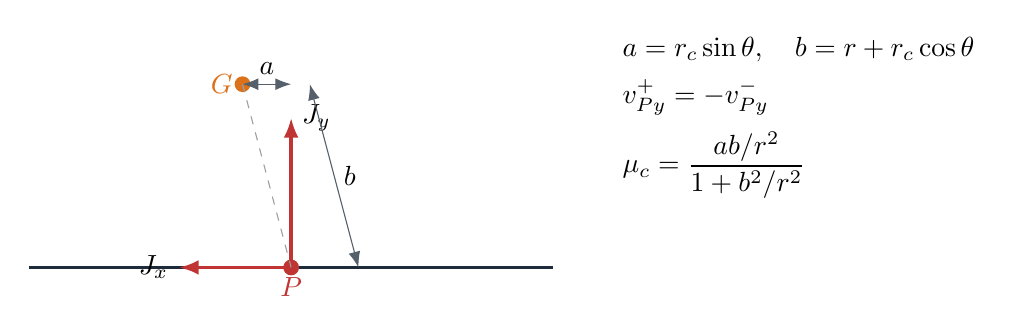
\begin{tikzpicture}[scale=.95]
  \draw[body] (-3.5,-1.8)--(3.5,-1.8);
  \coordinate (G) at (-.65,.65); \coordinate (P) at (0,-1.8);
  \fill[orange] (G) circle(3pt) node[left] {$G$};
  \fill[red] (P) circle(3pt) node[below] {$P$};
  \draw[force] (P)--++(0,2.0) node[right] {$J_y$};
  \draw[force] (P)--++(-1.5,0) node[left] {$J_x$};
  \draw[guide] (G)--(P);
  \draw[dim] (G)--($(G)+(.65,0)$) node[midway,above] {$a$};
  \draw[dim] ($(G)+(.9,0)$)--($(P)+(.9,0)$) node[midway,right] {$b$};
  \node[align=left,anchor=west] at (4.3,.2)
   {$a=r_c\sin\theta,\quad b=r+r_c\cos\theta$\\[5pt]
    $v_{Py}^+=-v_{Py}^-$\\[5pt]
    $\mu_c=\dfrac{ab/r^2}{1+b^2/r^2}$};
\end{tikzpicture}

% 9 question-05
\begin{tikzpicture}[x=1cm,y=1cm,font=\small]

\draw[body] (0,0)--(4.045,2.939);\draw[body] (0,0)--(4.045,-2.939);\draw[guide] (0,0)--(5,0) node[right] {$0^\circ$};\draw[blue,very thick] (2.427,-1.763) arc(-36:36:3);\draw (1,0) arc(0:36:1) node[midway,right] {$36^\circ$};\draw (1.3,0) arc(0:-36:1.3) node[midway,right] {$-36^\circ$};
\draw[orange,dashed] (0,0)--(-1.71,4.698);\node[orange] at (-1.7,5) {$\Theta$：约定的绝对像角};\node[align=left,anchor=west] at (6,1) {原图的观察角起点需另核实\\此图只声明镜像展开的角坐标\\形式像的位置不等同实际可见光路};

\end{tikzpicture}

% 10 solution-05
\begin{tikzpicture}[x=1cm,y=1cm,font=\small]

\draw[axis] (0,0)--(10,0) node[right] {$\Theta/36^\circ$};\draw[axis] (0,-1.6)--(0,1.8) node[above] {$\varphi/36^\circ$};\draw[blue,very thick] (1,1)--(3,-1)--(5,1)--(7,-1)--(9,1);\foreach \x in {1,3,5,7,9}{\node[below] at (\x,0) {$\x$};}\draw[guide] (0,1)--(9,1);\draw[guide] (0,-1)--(9,-1);
\node[align=center] at (4.8,2.8) {指定展开顺序的四个分支；开区间端点不纳入\\真实光路须另按观察位置与镜面有效侧筛选};

\end{tikzpicture}

% 11 question-06
\begin{tikzpicture}[x=1cm,y=1cm,font=\small]
\draw[axis] (0,0)--(9,0) node[right] {$W/W_0$};\draw[axis] (0,0)--(0,9) node[above] {$Q/W_0$};
\draw[blue,very thick] (0.000000,0.000000)--(2.000000,5.000000)--(5.000000,5.000000)--(4.333333,3.333333)--(3.333333,3.333333);
\fill (0.000000,0.000000) circle(2pt) node[above left] {$O$};
\fill (2.000000,5.000000) circle(2pt) node[above left] {$A$};
\fill (5.000000,5.000000) circle(2pt) node[above left] {$B$};
\fill (4.333333,3.333333) circle(2pt) node[above left] {$C$};
\fill (3.333333,3.333333) circle(2pt) node[above left] {$O_1$};
\node[align=left,anchor=west] at (9.2,3) {$OA\parallel BC$，$AB\parallel CO_1$\\[6pt]回到同一状态，但累计坐标继续增加\\[6pt]斜边对应恒定有效热容};
\end{tikzpicture}

% 12 solution-06
\begin{tikzpicture}[x=1cm,y=1cm,font=\small]
\draw[axis] (0,0)--(9,0) node[right] {$W/W_0$};\draw[axis] (0,0)--(0,9) node[above] {$Q/W_0$};
\draw[blue,very thick] (0.000000,0.000000)--(2.000000,5.000000)--(5.000000,5.000000)--(4.333333,3.333333)--(3.333333,3.333333);
\fill (0.000000,0.000000) circle(2pt) node[above left] {$O$};
\fill (2.000000,5.000000) circle(2pt) node[above left] {$A$};
\fill (5.000000,5.000000) circle(2pt) node[above left] {$B$};
\fill (4.333333,3.333333) circle(2pt) node[above left] {$C$};
\fill (3.333333,3.333333) circle(2pt) node[above left] {$O_1$};
\draw[orange,thick] (3.333333,3.333333)--(5.333333,8.333333)--(8.333333,8.333333)--(7.666667,6.666667)--(6.666667,6.666667);
\fill (8.333333,8.333333) circle(2pt) node[above right] {$B_1$};
\fill (7.666667,6.666667) circle(2pt) node[below right] {$C_1$};
\node[align=left,anchor=west] at (9.2,3) {$OA\parallel BC$，$AB\parallel CO_1$\\[6pt]回到同一状态，但累计坐标继续增加\\[6pt]斜边对应恒定有效热容};
\end{tikzpicture}

% 13 question-07
\begin{tikzpicture}[x=2cm,y=2cm,font=\small]
\draw[axis] (-1.5,0)--(2,0) node[right] {$x/r_0$};\draw[axis] (0,-1.3)--(0,2) node[above] {$y/r_0$};
\draw[very thick,blue] plot coordinates {(0.071937,0.243182) (0.065322,0.247155) (0.058540,0.250962) (0.051594,0.254599) (0.044488,0.258059) (0.037226,0.261336) (0.029812,0.264424) (0.022250,0.267317) (0.014546,0.270010) (0.006704,0.272496) (-0.001271,0.274770) (-0.009374,0.276827) (-0.017600,0.278660) (-0.025942,0.280265) (-0.034394,0.281637) (-0.042952,0.282770) (-0.051608,0.283660) (-0.060357,0.284302) (-0.069191,0.284690) (-0.078104,0.284822) (-0.087088,0.284692) (-0.096138,0.284297) (-0.105244,0.283631) (-0.114400,0.282693) (-0.123599,0.281478) (-0.132832,0.279982) (-0.142091,0.278203) (-0.151368,0.276138) (-0.160655,0.273784) (-0.169944,0.271138) (-0.179225,0.268199) (-0.188491,0.264964) (-0.197732,0.261431) (-0.206939,0.257599) (-0.216104,0.253467) (-0.225216,0.249033) (-0.234268,0.244298) (-0.243249,0.239259) (-0.252150,0.233917) (-0.260962,0.228273) (-0.269674,0.222326) (-0.278278,0.216077) (-0.286763,0.209527) (-0.295120,0.202677) (-0.303339,0.195529) (-0.311410,0.188085) (-0.319323,0.180345) (-0.327069,0.172314) (-0.334637,0.163994) (-0.342017,0.155387) (-0.349201,0.146497) (-0.356177,0.137328) (-0.362936,0.127883) (-0.369469,0.118167) (-0.375765,0.108185) (-0.381815,0.097942) (-0.387610,0.087442) (-0.393139,0.076691) (-0.398394,0.065696) (-0.403366,0.054462) (-0.408044,0.042996) (-0.412420,0.031304) (-0.416485,0.019395) (-0.420230,0.007276) (-0.423647,-0.005047) (-0.426727,-0.017564) (-0.429461,-0.030267) (-0.431843,-0.043147) (-0.433863,-0.056196) (-0.435514,-0.069403) (-0.436789,-0.082760) (-0.437680,-0.096257) (-0.438180,-0.109882) (-0.438283,-0.123626) (-0.437981,-0.137477) (-0.437270,-0.151426) (-0.436142,-0.165460) (-0.434592,-0.179567) (-0.432615,-0.193736) (-0.430205,-0.207955) (-0.427358,-0.222212) (-0.424070,-0.236493) (-0.420336,-0.250786) (-0.416152,-0.265078) (-0.411516,-0.279356) (-0.406424,-0.293606) (-0.400873,-0.307815) (-0.394861,-0.321968) (-0.388387,-0.336052) (-0.381448,-0.350053) (-0.374044,-0.363956) (-0.366175,-0.377748) (-0.357839,-0.391412) (-0.349037,-0.404935) (-0.339769,-0.418302) (-0.330038,-0.431497) (-0.319843,-0.444507) (-0.309188,-0.457315) (-0.298074,-0.469907) (-0.286504,-0.482268) (-0.274483,-0.494382) (-0.262013,-0.506235) (-0.249098,-0.517810) (-0.235745,-0.529094) (-0.221957,-0.540070) (-0.207741,-0.550723) (-0.193102,-0.561039) (-0.178049,-0.571002) (-0.162587,-0.580598) (-0.146724,-0.589812) (-0.130470,-0.598628) (-0.113831,-0.607033) (-0.096819,-0.615012) (-0.079442,-0.622551) (-0.061710,-0.629635) (-0.043634,-0.636251) (-0.025226,-0.642385) (-0.006497,-0.648024) (0.012541,-0.653154) (0.031875,-0.657762) (0.051492,-0.661836) (0.071379,-0.665363) (0.091521,-0.668331) (0.111904,-0.670728) (0.132513,-0.672544) (0.153333,-0.673766) (0.174347,-0.674384) (0.195539,-0.674388) (0.216893,-0.673768) (0.238392,-0.672514) (0.260018,-0.670617) (0.281752,-0.668069) (0.303577,-0.664862) (0.325474,-0.660986) (0.347424,-0.656437) (0.369407,-0.651206) (0.391403,-0.645288) (0.413393,-0.638677) (0.435355,-0.631368) (0.457270,-0.623356) (0.479115,-0.614638) (0.500871,-0.605210) (0.522514,-0.595069) (0.544024,-0.584213) (0.565377,-0.572641) (0.586553,-0.560352) (0.607528,-0.547345) (0.628280,-0.533622) (0.648786,-0.519183) (0.669022,-0.504030) (0.688967,-0.488165) (0.708596,-0.471591) (0.727887,-0.454314) (0.746816,-0.436336) (0.765359,-0.417664) (0.783494,-0.398304) (0.801197,-0.378261) (0.818445,-0.357545) (0.835213,-0.336162) (0.851480,-0.314123) (0.867221,-0.291437) (0.882414,-0.268114) (0.897036,-0.244166) (0.911064,-0.219604) (0.924476,-0.194443) (0.937248,-0.168694) (0.949360,-0.142373) (0.960788,-0.115495) (0.971512,-0.088075) (0.981510,-0.060131) (0.990761,-0.031679) (0.999245,-0.002738) (1.006940,0.026674) (1.013828,0.056537) (1.019889,0.086830) (1.025104,0.117532) (1.029454,0.148622) (1.032922,0.180077) (1.035490,0.211874) (1.037140,0.243989) (1.037857,0.276397) (1.037626,0.309073) (1.036429,0.341992) (1.034255,0.375126) (1.031087,0.408448) (1.026914,0.441932) (1.021723,0.475547) (1.015502,0.509266) (1.008241,0.543058) (0.999929,0.576894) (0.990557,0.610744) (0.980116,0.644575) (0.968600,0.678356) (0.956000,0.712055) (0.942312,0.745641) (0.927531,0.779079) (0.911652,0.812336) (0.894672,0.845379) (0.876589,0.878174) (0.857403,0.910687) (0.837113,0.942881) (0.815720,0.974724) (0.793226,1.006179) (0.769635,1.037211) (0.744949,1.067785) (0.719175,1.097865) (0.692318,1.127415) (0.664386,1.156399) (0.635388,1.184781) (0.605332,1.212525) (0.574231,1.239595) (0.542095,1.265956) (0.508938,1.291571) (0.474773,1.316404) (0.439617,1.340421) (0.403485,1.363585) (0.366396,1.385861) (0.328368,1.407215) (0.289421,1.427611) (0.249576,1.447015)};

\end{tikzpicture}

% 14 solution-07
\begin{tikzpicture}[x=2cm,y=2cm,font=\small]
\draw[axis] (-1.5,0)--(2,0) node[right] {$x/r_0$};\draw[axis] (0,-1.3)--(0,2) node[above] {$y/r_0$};
\draw[very thick,blue] plot coordinates {(0.071937,0.243182) (0.065322,0.247155) (0.058540,0.250962) (0.051594,0.254599) (0.044488,0.258059) (0.037226,0.261336) (0.029812,0.264424) (0.022250,0.267317) (0.014546,0.270010) (0.006704,0.272496) (-0.001271,0.274770) (-0.009374,0.276827) (-0.017600,0.278660) (-0.025942,0.280265) (-0.034394,0.281637) (-0.042952,0.282770) (-0.051608,0.283660) (-0.060357,0.284302) (-0.069191,0.284690) (-0.078104,0.284822) (-0.087088,0.284692) (-0.096138,0.284297) (-0.105244,0.283631) (-0.114400,0.282693) (-0.123599,0.281478) (-0.132832,0.279982) (-0.142091,0.278203) (-0.151368,0.276138) (-0.160655,0.273784) (-0.169944,0.271138) (-0.179225,0.268199) (-0.188491,0.264964) (-0.197732,0.261431) (-0.206939,0.257599) (-0.216104,0.253467) (-0.225216,0.249033) (-0.234268,0.244298) (-0.243249,0.239259) (-0.252150,0.233917) (-0.260962,0.228273) (-0.269674,0.222326) (-0.278278,0.216077) (-0.286763,0.209527) (-0.295120,0.202677) (-0.303339,0.195529) (-0.311410,0.188085) (-0.319323,0.180345) (-0.327069,0.172314) (-0.334637,0.163994) (-0.342017,0.155387) (-0.349201,0.146497) (-0.356177,0.137328) (-0.362936,0.127883) (-0.369469,0.118167) (-0.375765,0.108185) (-0.381815,0.097942) (-0.387610,0.087442) (-0.393139,0.076691) (-0.398394,0.065696) (-0.403366,0.054462) (-0.408044,0.042996) (-0.412420,0.031304) (-0.416485,0.019395) (-0.420230,0.007276) (-0.423647,-0.005047) (-0.426727,-0.017564) (-0.429461,-0.030267) (-0.431843,-0.043147) (-0.433863,-0.056196) (-0.435514,-0.069403) (-0.436789,-0.082760) (-0.437680,-0.096257) (-0.438180,-0.109882) (-0.438283,-0.123626) (-0.437981,-0.137477) (-0.437270,-0.151426) (-0.436142,-0.165460) (-0.434592,-0.179567) (-0.432615,-0.193736) (-0.430205,-0.207955) (-0.427358,-0.222212) (-0.424070,-0.236493) (-0.420336,-0.250786) (-0.416152,-0.265078) (-0.411516,-0.279356) (-0.406424,-0.293606) (-0.400873,-0.307815) (-0.394861,-0.321968) (-0.388387,-0.336052) (-0.381448,-0.350053) (-0.374044,-0.363956) (-0.366175,-0.377748) (-0.357839,-0.391412) (-0.349037,-0.404935) (-0.339769,-0.418302) (-0.330038,-0.431497) (-0.319843,-0.444507) (-0.309188,-0.457315) (-0.298074,-0.469907) (-0.286504,-0.482268) (-0.274483,-0.494382) (-0.262013,-0.506235) (-0.249098,-0.517810) (-0.235745,-0.529094) (-0.221957,-0.540070) (-0.207741,-0.550723) (-0.193102,-0.561039) (-0.178049,-0.571002) (-0.162587,-0.580598) (-0.146724,-0.589812) (-0.130470,-0.598628) (-0.113831,-0.607033) (-0.096819,-0.615012) (-0.079442,-0.622551) (-0.061710,-0.629635) (-0.043634,-0.636251) (-0.025226,-0.642385) (-0.006497,-0.648024) (0.012541,-0.653154) (0.031875,-0.657762) (0.051492,-0.661836) (0.071379,-0.665363) (0.091521,-0.668331) (0.111904,-0.670728) (0.132513,-0.672544) (0.153333,-0.673766) (0.174347,-0.674384) (0.195539,-0.674388) (0.216893,-0.673768) (0.238392,-0.672514) (0.260018,-0.670617) (0.281752,-0.668069) (0.303577,-0.664862) (0.325474,-0.660986) (0.347424,-0.656437) (0.369407,-0.651206) (0.391403,-0.645288) (0.413393,-0.638677) (0.435355,-0.631368) (0.457270,-0.623356) (0.479115,-0.614638) (0.500871,-0.605210) (0.522514,-0.595069) (0.544024,-0.584213) (0.565377,-0.572641) (0.586553,-0.560352) (0.607528,-0.547345) (0.628280,-0.533622) (0.648786,-0.519183) (0.669022,-0.504030) (0.688967,-0.488165) (0.708596,-0.471591) (0.727887,-0.454314) (0.746816,-0.436336) (0.765359,-0.417664) (0.783494,-0.398304) (0.801197,-0.378261) (0.818445,-0.357545) (0.835213,-0.336162) (0.851480,-0.314123) (0.867221,-0.291437) (0.882414,-0.268114) (0.897036,-0.244166) (0.911064,-0.219604) (0.924476,-0.194443) (0.937248,-0.168694) (0.949360,-0.142373) (0.960788,-0.115495) (0.971512,-0.088075) (0.981510,-0.060131) (0.990761,-0.031679) (0.999245,-0.002738) (1.006940,0.026674) (1.013828,0.056537) (1.019889,0.086830) (1.025104,0.117532) (1.029454,0.148622) (1.032922,0.180077) (1.035490,0.211874) (1.037140,0.243989) (1.037857,0.276397) (1.037626,0.309073) (1.036429,0.341992) (1.034255,0.375126) (1.031087,0.408448) (1.026914,0.441932) (1.021723,0.475547) (1.015502,0.509266) (1.008241,0.543058) (0.999929,0.576894) (0.990557,0.610744) (0.980116,0.644575) (0.968600,0.678356) (0.956000,0.712055) (0.942312,0.745641) (0.927531,0.779079) (0.911652,0.812336) (0.894672,0.845379) (0.876589,0.878174) (0.857403,0.910687) (0.837113,0.942881) (0.815720,0.974724) (0.793226,1.006179) (0.769635,1.037211) (0.744949,1.067785) (0.719175,1.097865) (0.692318,1.127415) (0.664386,1.156399) (0.635388,1.184781) (0.605332,1.212525) (0.574231,1.239595) (0.542095,1.265956) (0.508938,1.291571) (0.474773,1.316404) (0.439617,1.340421) (0.403485,1.363585) (0.366396,1.385861) (0.328368,1.407215) (0.289421,1.427611) (0.249576,1.447015)};
\fill (0.867733,0.893452) circle(2pt) node[right] {$P$};
\fill (-0.245163,0.238106) circle(2pt) node[left] {$C_\kappa$};
\draw[guide] (0.867733,0.893452)--(-0.245163,0.238106);
\draw[vec] (0.867733,0.893452)--(0.563280,1.410470);
\node[align=left,anchor=west] at (2.8,.8) {$\rho=r\sqrt{1+k^2}$\\[6pt]$\bm C_\kappa=kr\bm e_\theta$\\[6pt]$B(r)=B_0r_0/r$\\[6pt]箭头示例取 $q>0$、磁场入纸面};
\end{tikzpicture}

% 15 question-08
\begin{tikzpicture}[x=1cm,y=1cm,font=\small]
\draw[body] (0,0) ellipse(2.2 and 1.76);\fill[orange] (-1.32,0) circle(3pt) node[below] {原子核};\draw[guide] (-1.32,0) circle(2.2);\draw[axis] (-3.8,0)--(3.1,0);\node[above] at (0,2.6) {实线：椭圆；虚线：同能量圆轨道};
\end{tikzpicture}

% 16 solution-08
\begin{tikzpicture}[x=1cm,y=1cm,font=\small]
\draw[body] (0,0) ellipse(2.2 and 1.76);\fill[orange] (-1.32,0) circle(3pt) node[below] {原子核};\draw[guide] (-1.32,0) circle(2.2);\draw[axis] (-3.8,0)--(3.1,0);\node[above] at (0,2.6) {实线：椭圆；虚线：同能量圆轨道};\draw[dim] (-2.2,-.6)--(-1.32,-.6) node[midway,below] {$r_{\min}$};\draw[dim] (-1.32,-1.1)--(2.2,-1.1) node[midway,below] {$r_{\max}$};\draw[dim] (0,.3)--(2.2,.3) node[midway,above] {$a$};\node[align=left,anchor=west] at (4,1) {$a=r_n$，$e=\sqrt{1-l^2/n^2}$\\[6pt]核在焦点，圆心不在核处\\[6pt]$r_{\min,\max}=a(1\mp e)$};
\end{tikzpicture}
\end{document}
